\section{Appendix}
%\beginappendix
\subsection{Ablations}\label{sec:abla}
In this section we ablate and discuss some important design choice of OC-CLIP. We separately ablate and discuss : 
\begin{itemize}
    \item The \textbf{similarity score } coefficients $\alpha$ and $\beta$ that control the weight of the objects and relations in the global graph-image similarity score.
    \item \textbf{Binding module inductive biases} and their impact on compositional understanding performance. 
    \item \textbf{Local Loss} impact on downstream compositional
    understanding of relationships.
    \item \textbf{Layer selection} with OpenCLIP backbone.
\end{itemize}
\iffalse
Important ablation results are summarized in Table \ref{tab:ablation-results} and further commented below.
\begin{table}[htbp]
  \centering
  \new{
  \begin{tabular}{l|c|c|c|c|}
    \toprule
    Model & Loc Loss & Comp Att & Default Token & Relation Module  \\
    \midrule
    OC-CLIP & \checkmark & \checkmark & 4 & Additive  \\
    \hline
    - Loc Loss & -& \checkmark & 4 & Additive  \\
    \hline
    - Comp Att & \checkmark & - & 0 & Additive  \\
    \hline
    + Default Token (1)  & \checkmark & \checkmark & 1 & Additive  \\
    \hline
    \hline
    + MLP Relation & \checkmark & \checkmark & 4 & MLP  \\
    \hline
    \bottomrule
  \end{tabular}
    \begin{tabular}{l|c|c|c|c}
    \toprule
    Split & Swap Obj & Swap Att & Replace Att & Replace Rel \\
    \midrule
    Baseline & 80.7 & 88.7 & 88.3 & 80.6 \\
    \hline
    - Loc Loss & 73.1 & 88.3 & 89.2 & 74.7 \\
    \hline
    - Comp Att & 80.4 & 86.0 & 86.2 & 80.6 \\
    \hline
    + Default Token (1) & 79.9 & 88.4 & 86.7 & 80.9 \\
    \hline
    + MLP Relation & 78.4 & 87.8 & 87.1 & 78.7 \\
    \hline
    \bottomrule
  \end{tabular}}
  \caption{\new{Ablation Experiments, Fine-grained accuracy ($\%$ performance on representatitve SugarCrepe splits.}}
  \label{tab:ablation-results}
\end{table}
\fi

\paragraph{Similarity Score}
OC-CLIP's structured global similarity score is a combination of the object and relationship components respectively weighted by two learnt parameters $\alpha$ and $\beta$ balancing the different contributions. We let the model learn those parameters throughout the training. However, during preliminary experiments we tested a different combinations of initial coefficient within the [1.5, 1, 0.5, 0.1] grid and noticed that the model was always converging to a $\frac{\alpha}{\beta} \sim 3$ without any difference in the downstream compositional performance. We thus fix the initial coefficients to $\alpha=1.5$ and $\beta=0.5$ and treat them as parameters.

\paragraph{Default Token and Competitive Cross Attention}
In the binding module we propose to use an inductive biases to encourage the query tokens to attend to different groups of patches. In order to do so we use a competitive attention mechanism, the so called inverted cross attention common to many object-centric image encoder architecture \citep{locatello2020objectcentriclearningslotattention, WuInvertedAttentionTC}. We found that the use of inverted cross attention impacts slightly the fine-grained attribute binning performance (see ATT performance in Table~\ref{tab:ablation-main}), -Comp Att model does not use any inverted cross attention and is rather implemented with a regular cross attention mechanism, the softmax being done along the keys dimensions.). The finegrained attribute understanding (ATT) is affected by the absence of competitive attention between query slots going from 89.0\% to 85.9\% accuracy.

\paragraph{Local Graph Contrastive Loss} In designing the structured similarity score of OC-CLIP the relational component is formulated as the following cosine similarity $f_\phi(\mathbf{r}, \mathbf{S}^s, \mathbf{S}^o) = \text{cosine}(\mathbf{r}, f_s([\mathbf{r}, \mathbf{S}^s]) + f_o([\mathbf{r}, \mathbf{S}^o])$. In theory both $f_s([\mathbf{r}, \mathbf{S}^s]) $ and  $f_o([\mathbf{r}, \mathbf{S}^o]) $  can collapse to ignore the subject  object visual representation. In order to prevent such collapse we propose to add a local graph contrastive loss that shares similarity with hard-negative based learning. We enforce the model to model with a higher similarity the graph composed of the same nodes but with either swapped object and subject indices or shuffle objects and subjects indices within the local graph. In both of those cases the relation component of the structured similarity score becomes (for a single relation graph) : 
\begin{equation}
    \text{swap } \tilde{G}; \text{cosine}(\mathbf{r}, f_s([\mathbf{r}, \mathbf{S}^s]) + f_o([\mathbf{r}, \mathbf{S}^o])\\
\end{equation}
\begin{equation}
    \text{swap } \tilde{G}; \text{cosine}(\mathbf{r}, f_s([\mathbf{r}, \mathbf{S}^o]) + f_o([\mathbf{r}, \mathbf{S}^s])\\
\end{equation}
\begin{equation}
     \text{shuffle } \bar{G} ; \text{cosine}(\mathbf{r}, f_s([\mathbf{r}, \mathbf{S}^{j!=s}]) + f_o([\mathbf{r}, \mathbf{S}^{i!=o}])
\end{equation}
This prevents the model from collapsing because  ground-truth $G$ is distinguishable from $\tilde{G}$ and $\bar{G}$ only if the visual representations are not ignored in the relationships components.
As shown in Table~\ref{tab:ablation-main}, removing the local loss effectively impacts downstream relational understanding on SugarCrepe with a REL accuracy decreasing from $80.5$ to $72.8$ hence showing the effectiveness of the local graph contrastive loss.

% \vspace{-20pt}
\iffalse
\begin{figure}[ht]
\centering
    \begin{subfigure}[b]{0.2\textwidth}
        \centering    
    \includegraphics{figures/ablation_task_coef_swap_att.pdf}
        \caption{Swap Att}
    \end{subfigure}%
    \hfill
    \begin{subfigure}[b]{0.2\textwidth}
        \centering    \includegraphics[height=1in]{figures/ablation_task_coef_swap_obj.pdf}
        \caption{Swap Obj}
    \end{subfigure}%
    \hfill
    \begin{subfigure}[b]{0.2\textwidth}
        \centering    \includegraphics[height=1in]{figures/ablation_task_coef_replace_obj.pdf}
        \caption{Replace Obj}
    \end{subfigure}%
    \hfill
    \begin{subfigure}[b]{0.2\textwidth}
        \centering    \includegraphics[height=1in]{figures/ablation_task_coef_replace_att.pdf}
        \caption{Replace Att}
    \end{subfigure}%
    \hfill
    \begin{subfigure}[b]{0.19\textwidth}
        \centering    \includegraphics[height=1in]{figures/ablation_task_coef_replace_rel.pdf}
        \caption{Replace Rel}
    \end{subfigure}%
  \caption{ \textbf{Local Perturbed Graphs Ablation} In this ablations we keep the initialization seed fixed and include a perturbed graph as a negative sample inside the loss by swapping the order of the subject and object (y-axis), $\bar{G}$ or sampling random subject and object within the positive scene graph (x-axis), $\tilde{G}$.}
  \label{fig:abla_coefs}
\end{figure}
\fi

\paragraph{Scoring dimensionality} Our structured similarity score allows the text encoder to focus on encoding information about individual objects and their relationships, rather than the entire scene configuration. To achieve this, we experimented with different dimensionality for both the object scoring bottleneck and the relationship scoring bottleneck. Specifically, each of these scores is designed as a cosine distance between a text representation and a visual component (as described in Section \ref{sec:our_score}), with each operating at a bottleneck dimension of $d_{\text{obj}}$ and $d_{\text{rel}}$. In contrast, OpenCLIP represents both the scene caption and the visual representation at a shared dimension of $d=512$. We expect that our model can operate effectively at a much lower dimensionality, as it requires less capacity to encode single objects and relationships. We present an ablation study of these two dimensions in Figure \ref{fig:abla_dim} and notice that our model is quite robust when we operate on lower dimensional space (eg. 128). We use this results to scale our experiments and train the model from scratch with a smaller text encoder as explained in the next section~\ref{sec:scale} corresponding to experiments shown in Section \ref{sec:noisy}.
\paragraph{Layer Selection} Previous work focusing on dense segmentation tasks\citep{xu2022groupvitsemanticsegmentationemerges} show that taking features from earlier layer in CLIP's ViT help with fine-grained tasks. Here we ablate OC-CLIP's version using the OpenCLIP pretrained backbone when inserting the binding module after layer $L-k$ for $k \in [0..4]$, 0 being the last layer. Results on merged Sugarcrepe splits are given in Figure~\ref{fig:layers}. The object related queries seem to decrease as a function of $k$ where as the replace rel split is increasing with k. To that end, we actually insert our binding module after layer $L-2$, where $L$ is the index of the last transformer layer of the ViT.
\begin{figure}
    \centering
    \includegraphics[width=\textwidth]{figures/layers_abla.png}
    \caption{ViT features layer ablation.}
    \label{fig:layers}
\end{figure}

\begin{figure}[ht]
\centering
    \begin{subfigure}[b]{0.19\textwidth}
        \centering    \includegraphics[height=1in]{figures/swap_att_final.png}
        \caption{Swap Att}
    \end{subfigure}%
    \hfill
    \begin{subfigure}[b]{0.19\textwidth}
        \centering    \includegraphics[height=1in]{figures/swap_obj_final.png}
        \caption{Swap Obj}
    \end{subfigure}%
    \hfill
    \begin{subfigure}[b]{0.19\textwidth}
        \centering    \includegraphics[height=1in]{figures/replace_obj_final.png}
        \caption{Replace Obj}
    \end{subfigure}%
    \hfill
    \begin{subfigure}[b]{0.19\textwidth}
        \centering    \includegraphics[height=1in]{figures/replace_att_final.png}
        \caption{Replace Att}
    \end{subfigure}%
    \hfill
    \begin{subfigure}[b]{0.19\textwidth}
        \centering    \includegraphics[height=1in]{figures/replace_rel_final.png}
        \caption{Replace Rel}
    \end{subfigure}%
  \caption{\textbf{Score dimensionality ablations} In this ablations we keep the initialization seed fixed and vary the dimensionality of the relation score $d_{\text{rel}}$ (x-axis) and object score $d_{\text{obj}}$(y-axis) and report the performance on the swap and replace splits of sugarcrepe.}
  \label{fig:abla_dim}
\end{figure}


% \subsection{0-shot classification results}
% See Table~\ref{suppl:tab:classification}
% \begin{table}[ht]
% \centering
% \resizebox{\textwidth}{!}{%
% \begin{tabular}{@{}llccccccccccccccc@{}}
% \toprule
% \multirow{2}{*}{\textbf{Model}} & \multirow{2}{*}{\textbf{FT data}} & \multicolumn{1}{l}{\multirow{2}{*}{\textbf{\# ep}}} & \multicolumn{6}{c}{\textbf{Linear eval w/ bbone feature}} & \multicolumn{6}{c}{\textbf{Linear eval w/ B_k}} & \multicolumn{2}{c}{\textbf{0-shot SugarCrepe}} \\ \cmidrule(l){4-9} \cmidrule(l){10-15} \cmidrule(l){16-17}
%  &  & \multicolumn{1}{l}{} & \textbf{ImageNet\textsubscript{1K}} & \textbf{cifar10} & \textbf{cifar100} & \textbf{CLEVR Count} & \textbf{CLEVR Dist} & \textbf{Eurosat} & \textbf{ImageNet\textsubscript{1K}} & \textbf{cifar10} & \textbf{cifar100} & \textbf{CLEVR Count} & \textbf{CLEVR Dist} & \textbf{Eurosat} & \textbf{Swap obj.} & \textbf{Swap att.} \\ \midrule 
% clip & - & - & 71.4 & 65.0 & 43.9 & 44.8 & 48.8 & 88.0 & - & - & - & - & - & - & 68.2 & 66.2 \\
% clip & cc12m & 10 & 72.7 & 67.5 & 44.8 & 45.0 & 47.3 & 87.9 & - & - & - & - & - & - & 71.9 & 70.8 \\
% oc-clip & coco & 99 & 73.3 & 70.9 & 48.3 & 49.1 & 54.3 & 89.7 & 62.3 & 58.4 & 38.4 & 42.1 & 45.1 & 84.5 & 75.5 & 85.5 \\
% oc-clip & cc12m & 10 & 73.2 & 70.5 & 48.8 & 49.3 & 54.2 & 90.2 & 66.2 & 62.0 & 40.1 & 43.0 & 45.1 & 84.9 & 73.7 & 85.3 \\
%  &  & 15 & 73.4 & 71.5 & 49.0 & 49.9 & 53.5 & 90.0 & 66.2 & 63.0 & 41.3 & 44.1 & 45.5 & 85.2 & 73.2 & 85.7 \\ \bottomrule
% \end{tabular}%
% }
% \caption{\textbf{Transferability to image classification benchmarks.}}
% \label{suppl:tab:classification}
% \end{table}



\subsection{Experiments on CC3M/12M.}\label{sec:scale}
\new{In the compositional understanding experiments we compare our approach with data-centric finetuning methods that do not add any additional parameters. These methods are expected to retain some of the general capabilities of the initial backbone. In contrast, our binding  and relationship modules is trained from scratch, which means it may not generalize as well to unseen data and can only be expected to work well within the vocabulary domain it has been exposed to (eg. COCO/VG/GQA in our experiments setting). 
However an interesting question would be to asses whether such inductive biases and structured similarity object might have some sclaing potential on noisy and non human curated datasets such as CC12M \citep{changpinyo2021cc12m}. To answer that question we propose to train both CLIP and OC-CLIP architectures from scratch on combinations of CC3M,  CC12M and CC3M+12M and compare both of their general understanding and compositional downstream performance.
In addition to the zero-shot evaluation, we also provide a computational analysis of the binding module to gain insights into its behavior and limitations.

\paragraph{Training Details}

 In order to show the potential of OC-CLIP to learn from scene-graph obtained from a non human-curated captioning dataset we train both ViT-B-16 OpenCLIP model and OC-CLIP from scratch on CC3M~\citep{sharma-etal-2018-conceptual}, CC12M~\citep{changpinyo2021cc12m} and the merge of both (15M) . We did not tune the hyperparameters and used the same hyperparameters as suggested in \citep{mu2021slipselfsupervisionmeetslanguageimage}. Both models are trained for 5, 15, and 25 epochs, using a batch size of 4096, a learning rate of $1e-3$, 2k steps learning rate warmup and a cosine decay after. As recommended by \citet{mu2021slipselfsupervisionmeetslanguageimage} we used AdamW optimizer with 0.5 of weight decay and $\beta_2$ set to 0.98.We report extensive zero-shot downstreeam classification performance on the ELEVATER \citep{li2022elevaterbenchmarktoolkitevaluating} suite in Table \ref{tab:classification-downstream}. We did not use any templates and use raw labels instead. Both models were trained using 4x8 V100 GPUS with a local batch size of 128. OC-CLIP shows  performance gains in both zero-shot classification (a notable +12.7\% in ImageNet) when trained on the same setting.  These experiments show that the structured training of OC-CLIP can scale to automatic alt-text captioning dataset. We leave further scaling for future work as the main focus of our work is to emphasize the binding problem that arises when using a vector-based representation and a set of inductive biases  as a way of operating on a more structured representation (eg. scene graph).
\begin{table*}
\setlength{\tabcolsep}{2pt}
\linespread{1}
\scriptsize
\begin{adjustbox}{width=\textwidth}
\new{    
\begin{tabular}{ll ccccccccccccccccccccccc|c} &&
\rotatebox[origin=lb]{90}{\smash{Food-101}} & \rotatebox[origin=lb]{90}{\smash{CIFAR-10}} & \rotatebox[origin=lb]{90}{\smash{CIFAR-100}} & \rotatebox[origin=lb]{90}{\smash{SUN397}} & \rotatebox[origin=lb]{90}{\smash{Cars}} & \rotatebox[origin=lb]{90}{\smash{Aircraft}} & \rotatebox[origin=lb]{90}{\smash{DTD}} & \rotatebox[origin=lb]{90}{\smash{Pets}} &  \rotatebox[origin=lb]{90}{\smash{FER-2013}} & \rotatebox[origin=lb]{90}{\smash{STL-10}} & \rotatebox[origin=lb]{90}{\smash{EuroSAT}} &
\rotatebox[origin=lb]{90}{\smash{RESISC45}} & \rotatebox[origin=lb]{90}{\smash{GTSRB}} & \rotatebox[origin=lb]{90}{\smash{KITTI}} & \rotatebox[origin=lb]{90}{\smash{Country211}} & \rotatebox[origin=lb]{90}{\smash{PCAM}} &
\rotatebox[origin=lb]{90}{\smash{UCF101 Frames}} & \rotatebox[origin=lb]{90}{\smash{CLEVR}} & \rotatebox[origin=lb]{90}{\smash{HatefulMemes}} & \rotatebox[origin=lb]{90}{\smash{MNIST}} & \rotatebox[origin=lb]{90}{\smash{SST2}} &
\rotatebox[origin=lb]{90}{\smash{ImageNet}} \\%& \rotatebox[origin=lb]{90}{\smash{Average}}  \\
\hline
\multirow{2}{1em} & CLIP (3m) & 12.8 & 44.9 & 19.9& 27.9 & 1.2 & 1.3 & 9.7 & 12.6 &1.3 &76.1 & 15.8 & 13.5 & 6.9 & 24.9 & 0.6 & 44.3 & 17.8 & 11.1 & 51.2 &7.8& 47.4 & 13.9  \\
& OC-CLIP (3m)  & 15.3 & 57.1 & 24.8 & 33.1 & 1.2 & 1.6 & 13.3& 16.3 & 9.9&82.0 & 16.2 & 22.0 & 4.5 & 30.8 & 0.7 & 55.6 & 22.5 & 12.5 & 52.0 &11.6& 50.1 & \textbf{19.2}  \\
\hline
\multirow{2}{1em} & CLIP (12m) & 42.7 & 63.2 & 30.2 & 42.7 & 15.5 & 3.1 & 14.5 & 52.6 &13.1 &85.7 & 12.3 & 28.5 & 8.3 & 34.9 & 3.9 & 54.4 & 33.9 & 11.8 & 51.4 &11.2& 51.9 & 30.5  \\
& OC-CLIP (12m)  & 54.1 & 74.5 & 44.6 & 51.4 & 21.1 & 3.7 & 19.4 & 66.4 & 7.4&91.9 & 31.8 & 40.6 & 8.1 & 41.9 & 5.9 & 56.1 & 45.7 & 12.7 & 49.2 &9.7& 50.2 & \textbf{42.3}  \\
\hline
\multirow{2}{1em} & CLIP (15m) & 43.4 & 72.3 & 33.8 & 44.2 & 15.8 & 2.3 & 14.0 & 53.8 &9.2&89.1 & 24.0 & 30.0 & 11.0 & 28.0 & 3.3 & 50.1 & 37.4 & 12.5 & 50.6 &10.2& 50.1 & 32.2  \\
& OC-CLIP (15m)  & 54.5 & 82.3 & 46.6 & 54.1 & 20.2 & 3.7 & 22.1 & 69.2 & 5.2&94.2 & 26.8 & 44.4 & 9.4 & 29.9 & 5.9 & 52.9 & 47.3 & 14.5& 51.3 &9.0& 49.9 & \textbf{45.0}  \\
\hline
\end{tabular}}



\end{adjustbox}
\caption{Zero-shot evaluation of CLIP vs OC-CLIP. Trained on varying size of data ( cc3m, cc12m, merged 15m) for 25 epochs.}
\label{tab:classification-downstream}

\end{table*}

\paragraph{Computational analysis of OC-CLIP} In OC-CLIP the visual and text modalities representations are no longer independent (as opposed to CLIP). A image representation is the results of some text-conditioned mechanism operated by the binding module. It essentially extracts relevant visual slots that constitutes the nodes of the scene graph coming from the caption. As a result, there is some notable computational overhead introduced by the additional cross-attention operations of the binding module. In particular : \begin{itemize}
    \item  1. The text encoder needs to encode the $N$ nodes and $R$ relations of the scene graph as opposed to a single sentence encoding in CLIP.
    \item 2. For each Image-Graph pair, The $N$ text nodes cross-attends to $N_{im}$ patches of the ViT in order to extract the structured visual slots.
\end{itemize}
When training OC-CLIP from scratch we propose to mitigate those two overheads respectively by : 
\begin{itemize}
    \item 1. Using a smaller embedding width (256 vs 512) and number of layers (6 vs 12) in the text encoder. Indeed OC-CLIP only need to encode information about objects and relationships and we expect such encoding to require much less capacity than an encoder that needs to encode a whole caption composed of multiple objects and relations between them.
    \item 2. We operate on a reduced embedding space 256 for the binding module and thus first project the ViT-B-16 patches from a 768 to a 256 embedding space before computing the nodes to patch cross attention logits.
    \item 3. We use the SigLip~\citep{zhai2023sigmoidlosslanguageimage} loss to make efficient use of batch chunking and gradient checkpointing.
\end{itemize}
We only perform experiments with a B-16 architecture for the ViT but perform the computational analysis fro both B and L backbones. We report the results in Table \ref{tab:vit-scale-binding-module} We note that there is  a significant overhead with a base architecture 2.2x but since the binding module perform the same number of operations no matter what the ViT is we show that when scaling the ViT backbone, the binding module is not the bottleneck anymore and the computational overhead is reduced (1.3x).
\begin{table}[htbp]
  \centering
  \begin{adjustbox}{width=\textwidth}
  \new{
  \begin{tabular}{|c|cc|ccc|c|}
    \hline
    Model & ViT Backbone & Text (w,l,ctx) & Binding Module GFLOPs  & Text GFLOPS & Vision GFLOPs & Total GFLOPs\\
    \hline
    OC-CLIP & B &(256, 6, 20)&12(*num workers) &180 & 1k& 2.2x \\
    CLIP & B & (512, 12, 77)& -& 186& 1k& 1x\\
    \hline
    OC-CLIP& L &(256, 6, 20)& 12(*num workers)& 180&4.9k& 1x \\
    CLIP& L&(512, 12, 77)& - & 186 &4.9k& 1.3x\\
    \hline
  \end{tabular}}
  \end{adjustbox}
  \caption{\new{Computational Comparison of CLIP and OC-CLIP. Calculations are made for a local batch size (per GPU) of 64. We give the Total GFLOPs based on a global batch size of 8192 (=128 num workers). When scaling the ViT backbone the computational overhead of the binding module remains fixed and is not the main bottleneck anymore.}}
  \label{tab:vit-scale-binding-module}
\end{table}
\subsection{Scene Graph Parsing Discussion}\label{app:parsing}
\paragraph{Comparison of different parsing methods} Although the parsing method is not the core of our contribution we provide here a couple of qualitative and quantitative comparisons to motivate the choice of using an LLM to perform the parsing of the captions despite the pre-processing computational overhead it entails. We identify 3 families of parsing method that operate on text-only input and provide insights on their respective : 
\begin{itemize}
    \item \textbf{Automatic parsing methods} : method based on hand-crafted rules about the semantics in order to extract tags and more complex dependency graphs. TagAlign also compares to nltk and justifies the choice of going to an llm-based method. We consider a representative of those automatic parsing methods based on spacy \citep{spacy2}.
    \item \textbf{Finetuned factual scene graph parser} trained in a supervised way to extract scene graph. We consider a representative of them, a state-of-the-art factual scene graph parser based on T5 model \citep{li2023factualbenchmarkfaithfulconsistent} trained to extract fine-grained scene graph information about the objects and relations in an input caption.
    \item \textbf{LLM-based}, here we choose llama3-8b as a representative and leave the extensive analysisof the bias/cues of different llm families of model for future work.
\end{itemize}
We identified failures modes of automatic parsing and finetuned that are relevant to compositional understanding of clip-like models and justify the use of an llm-based parsing method and summarize them in Table \ref{tab:parsing-errors}. We show on one hand that automatic parsing methods are prone to oversimplification, missing relations and mistaking an attribute modifiers with an object. On the other hand supervised scene graph parser seems to be prone to relation classification error and important atteibute binding error when the different objects mentioned in a caption share the same label tag.


\begin{table}[htbp]
  \centering
  \small
  \begin{adjustbox}{width=\textwidth}
  \new{
  \begin{tabular}{|l|l|l|l|}
    \hline
    \textbf{Caption} & \textbf{Spacy} & \textbf{T5} & \textbf{LLM} \\
    \hline
    A brown cat is lying on a computer & 
      \begin{tabular}{@{}l@{}}
        Objects: a brown cat, a computer \\
        Relations: \{\textcolor{red}{on}, 0, 1\} \quad \textcolor{red}{(Oversimplification error)}
      \end{tabular} &
      \begin{tabular}{@{}l@{}}
        Objects: brown cat, computer \\
        Relations: \{\textcolor{red}{lay on}, 0, 1\} \quad \textcolor{red}{(Relation classification error)}
      \end{tabular} &
      \begin{tabular}{@{}l@{}}
        Objects: brown cat, computer \\
        Relations: \{lying on, 0, 1\}
      \end{tabular} \\
    \hline
    A man is on the left of the dog & 
      \begin{tabular}{@{}l@{}}
        Objects: a man, \textcolor{red}{the left}, a dog \quad \textcolor{red}{(Wrong POS)} \\
        Relations: \{\textcolor{red}{of}, 1, 2\} \quad \textcolor{red}{(Missing relation)}
      \end{tabular} &
      \begin{tabular}{@{}l@{}}
        Objects: man, dog \\
        Relations: \{at the left of, 0, 1\}
      \end{tabular} &
      \begin{tabular}{@{}l@{}}
        Objects: man, dog \\
        Relations: \{on the left of, 0, 1\}
      \end{tabular} \\
    \hline
    A woman in blue and a woman in red & 
      \begin{tabular}{@{}l@{}}
        Objects: a woman, \textcolor{red}{red}, a woman,  \quad \textcolor{red}{(Wrong POS)} \\
        Relations: \{, 0, 1\}, \{in, 0, 2\}, in, 2, 3\} 
      \end{tabular} &
      \begin{tabular}{@{}l@{}}
        Objects: \textcolor{red}{blue red clothes}, woman \quad \textcolor{red}{(Wrong attribute binding)}\\
        Relations: \{wear, 0, 1\} 
      \end{tabular} &
      \begin{tabular}{@{}l@{}}
        Objects: woman in red, woman in blue \\
        Relations: \{\}
      \end{tabular} \\
    \hline
  \end{tabular}}
  \end{adjustbox}
  \caption{\new{Comparison of parsing errors made by different parsers.}}
  \label{tab:parsing-errors}
\end{table}

We additionally train OC-CLIP on COCO captions parsed by those 3 different parsing models and compare the downstream compositional understanding performance in Figure \ref{fig:parsing-perf}. Coherent with the qualitative analysis the choice of the parsing family mostly impact relational understanding. We observe for the SugarCrepe swap object (replace rel resp.)  a decrease of $9.3\%$ (resp. $14.1\%$) for spacy and $3.4\%$ (resp. $6.3\%$) for a supervised T5 model  as compared to OC-CLIP on scene graphs extracted by llama3-8b. 
Close to our work, TagAlign\citep{liu2024tagalignimprovingvisionlanguagealignment} also quantitatively and qualitatively analyze the objects tags than can be extracted with an nltk-based and llm-based parser and show that training CLIP with an additional object and attribute tag classification loss with tags coming from an llm results in better downstream zero-shot semantic segemntation.
\begin{figure}
    \centering
    \includegraphics[width=\linewidth]{figures/parsing_performances.png}
    \caption{\new{Downstream Compositional Understanding of OC-CLIP when trained on different parsing of COCO-Captions.}}
    \label{fig:parsing-perf}
\end{figure}



\paragraph{Limitations of LLM-based parsing for OC-CLIP}
We also acknowledge that using and LLM as a parser may also have some limitations and evaluating the impact of the downstream performance of different LLMs or VLMs is an interesting question. In particular, llm-based parsing might not extract accurate scene graphs, especially when the dependency between the objects in a captions is rather complex or ambiguous. And informing the parser in prompt with visual information might be an interesting direction. However the exact instanciation of the LLM-based parser used is orthogonal to our contribution and we leave this analysis for future work.


\paragraph{Scene Graph Parsing cost}
We performed the parsing by serving instances of Llama3.1-8b on v100 GPUs. Each datasets is then chunked in $N$ process that do not require any GPUs and send requests to the served LLM parsers through vllm\footnote{https://github.com/vllm-project/vllm} to maximize the throughput of the parallelized requests. For reference we parsed the COCO datasets ($\sim$ 500k captions) parallelizing 10 instances of the parser, and with 128 chunks in 3.5 hours and Visual-Genome ($\sim$ 200k captions) with 8 instances, 64 chunks in 1.7hours. The parsing time can further be optimized by serving more instances, using more performant GPUs (A100, H100 etc..), serving each instance in parallel in more GPUs to maximized the number of requests that can be processed per second.
For the cc3m and cc12m, in order to accelerate the parsing, we kept the LLM parser local using ollama\footnote{https://ollama.com/} on v100 GPUs. CC3M was chunked into 500 and CC12M into 1000 smaller chunks, we launched the jobs sequentially. CC12M took about ~3days to parse but could likewise be accelerated using faster GPUS.

}

\subsection{Additional Compositional Understanding results}\label{app:vl}
Our main goal is to evaluate CLIP-like models compositional understanding in plausible and grammatically correct cases. \citet{hsieh2023sugarcrepefixinghackablebenchmarks} have identified exploitable textual biases in previous mainstream procedurally-generated hard negatives benchmarks like the COCO and Flickr set of ARO and VL-checklist. Specifically they show that procedurally generated hard negatives are either highly grammatically incorrect and can be identified by a blind model or by a good language model that can measure the plausibility of the caption. The SugarCrepe is thus designed to  pfollow the same fine-grained taxonomy on attributes, objects, relationships as VL-checklist but ensures that the hard-negative are not distinguishable by a blind model. The main results of our paper thus focus on this benchmark. We however also give the performance of our model on the full ARO suite and VL-Checklist in Table~\ref{tab:vl_aro} for reference.  
\begin{table}[htbp]
\begin{small}
\begin{sc}
\resizebox{\textwidth}{!}{
\begin{tabular}{lcccccccc}

\toprule
Model & \multicolumn{3}{c}{VL-Checklist} & \multicolumn{4}{c}{ARO} \\
\cmidrule(lr){2-4}
\cmidrule(lr){5-8} 
& Object & Relation   & Attribute & Attribution & Relation & COCO-order & Flickr-order \\
\midrule
CLIP & 80.0 & 63.0&  67.4& 63.2& 60.0 & 47.9 & 60.2 \\
BLIP & 82.2 & 70.5 &  75.2& 63.2& 60.0 & 47.9 & 60.2 \\
XVLM & 85.8 & 70.4 &  75.1& 73.4& 86.8 & - & -\\
\midrule
\textit{Hard-negative Methods} \\
CLIP-SVLC &85.0 & 68.9.7 & 72.0 & 73.0 & 80.6 & 84.7 & 91.7 \\
NegCLIP& 84.1& 63.5& 70.9 & 71 & 81 & 86 & 91 \\
CE-CLIP& 84.6 &71.8 &  72.6& 76.4 & 83.0 & - & - \\
\textit{Dense captioning+Hard-Negative} \\
DAC-LLM$_\text{500k}$ & 66.5 & 56.8 & 57.4 & 63.8 & 60.1 & 50.2 & 61.6 \\
DAC-LLM$_\text{3M}$ & 87.3 & 86.4  & 77.3 & 73.9 & 81.3 & 94.5 & 95.7 \\
DAC-SAM$_\text{3M}$ & 88.5 & 89.7 & 75.8 & 70.5 & 77.2 & 91.2 & 93.9 \\  
DCI & 80.7& 70.1 & 68.7 & 67.6 & 76.2 & 88.6 & 91.3 \\
DCI$_\text{neg}$ & 88.4 & 61.3 & 70.4 & 62.0 & 57.3 & 39.4 & 44.6\\
\midrule
OC-CLIP & 90.7 & 80.0 & 75.6 & 84.0 & 84.9 & 94.2 & 84.8 \\
\bottomrule
\end{tabular}
}
\end{sc}
\end{small}


\caption{\new{Results (\%) on VL-Checklist  and ARO Benchmark.}}
\label{tab:vl_aro}
\end{table}
\subsection{PUG Dataset }\label{sec:pug_app}
In this section we describe in more details the content of the synthetic experiments, give more context on the motivation along with additional results. 
\paragraph{Motivation}The rise of data-centric hard negative methods were motivated by the bag-of-words behaviour \citep{yuksekgonul2023when} of CLIP noticed in "simple swap-attribute" retrieval tasks. Hard-negative methods propose to mitigate this behaviour by finetuning CLIP-like models  on data points with minimal changes but semantically different meanings. However we experimentally observed that all the methods fail to increase performance specifically in swap attribute kind of splits. In order to further isolate the root cause, we propose a series of synthetic experiments that compare covering more hard-negative data points with OC-CLIP on varying proportion of training samples and hard-negative samples. By restricting the environment to a closed-set vocabulary of backgrounds, attributes, and object classes, we can enumerate all possible hard-negatives, allowing us to systematically evaluate the effectiveness of different approaches.
Our results show that simply \emph{adding more hard-negatives plateaus and is not sample-efficient, as the swap attribute binding performance always underperforms OC-CLIP trained on less data without any hard-negatives} in a simple object-attribute binding task \ref{fig:binding_pug}. However, when combined with OC-CLIP inductive bias, hard-negatives complementarily improve downstream performance. This suggests that our model, OC-CLIP, is a more sample-efficient approach to addressing the bag-of-words behavior of CLIP models.
We hypothesize that the root cause of this issue thus lies in the representation format used in CLIP's original formulation, which relies on a single vector to capture complex semantic relationships. Our proposed method introduces inductive biases that allow the model to learn more structured representations, avoiding superposition of features \citep{greff2020bindingproblemartificialneural} and effectively mitigating the bag-of-words behavior. Through these synthetic experiments, we demonstrate the effectiveness of our approach and provide insights into the sample-efficiency limitations of existing data-centric methods.

\paragraph{Dataset splits} The synthetic experiments we propose are based on  the controlled 3D environment  PUG~\citep{bordes2023pugphotorealisticsemanticallycontrollable}. We operate in a 3D envrionment with pairs or single textured animals in different backgrounds. The factors of variation are :
\begin{itemize}
    \item \textbf{5 Backgrounds} : desert, arena, ocean floor, city, circus
    \item \textbf{20  Animals}  : goldfish, caribou, elephant, camel, penguin, zebra,
        bear, crocodile, armadillo, cat, gecko, crow,
        gianttortoise, rhinoceros, dolphin, lion, orca, pig,
        rabbit, squirrel
    \item \textbf{4 textures} : red, white, asphalt, grass
    \item \textbf{2 spatial constraints} for pairs : left/right, above/under
\end{itemize}
The different splits 
We then construct splits that aim at evaluating separately attribute binding and spatial relationships understanding. In all the different splits, we include images with single animals in all the possible \emph{background-texture-animal} conjunctions.
\paragraph{Attribute Binding Splits} The attribute binding training and testing splits are constructed as follows : (1) - We list all the possible pairs of animals,(2) - We randomly  and i.i.d. select a percentage \%  $N_{\text{train}}$ of pairs to include in the train split, (3) - For each training pair we select a pair of assigned attribute (for example if cat and caribou are in the train split we will assign red to cat and white to caribou and will remove all the other attribute-animal conjunction from the training. This is done such that we can control for the \emph{replace attribute} hard negative presence. (4) - For each pair in the training set we separate the corresponding hard negative examples with the same bag of words but swapped attributes (referred to as \emph{Seen Pairs} in Figure \ref{fig:abla_attr}) and the same pair but a different bag of words ( referred to as \emph{Different Bag-of-words} in \ref{fig:abla_attr})  , (5) - finally we also isolate unseen pairs of animals. We also include the accuracy on the training pairs that do not have their corresponding hard negatives in the test set).
\begin{figure*}[ht]
\centering
    \begin{subfigure}[b]{0.15\textwidth}
        \centering    \includegraphics[width=0.9\textwidth, keepaspectratio]{figures/pairs.pdf}
        \caption{\tiny{} Pairs  }
    \end{subfigure}%
    % \hfill
    \begin{subfigure}[b]{0.2\textwidth}
        \centering    \includegraphics[width=0.9\textwidth,  keepaspectratio]{figures/pairs_0.pdf}
        \caption{\tiny{} Train Pairs}
    \end{subfigure}%
    \hfill
    \begin{subfigure}[b]{0.2\textwidth}
        \centering    \includegraphics[width=0.9\textwidth,  keepaspectratio]{figures/pairs_1.pdf}
        \caption{\tiny{} Seen Pairs}
    \end{subfigure}%
    \hfill
    \begin{subfigure}[b]{0.2\textwidth}
        \centering    \includegraphics[width=0.9\textwidth,  keepaspectratio]{figures/pairs_2.pdf}
        \caption{\tiny{} Different Bag-of-words}
    \end{subfigure}%
    \hfill
    \begin{subfigure}[b]{0.2\textwidth}
        \centering    \includegraphics[width=0.9\textwidth, keepaspectratio]{figures/pairs_3.pdf}
        \caption{\tiny{} Unseen Pairs}
    \end{subfigure}%

    \begin{subfigure}[b]{0.15\textwidth}
        \centering    \includegraphics[width=\textwidth,  keepaspectratio]{figures/single.pdf}
        \caption{\tiny{} Single Object }
    \end{subfigure}%
    \begin{subfigure}[b]{0.2\textwidth}
        \centering    \includegraphics[width=\textwidth, keepaspectratio]{figures/single_0.pdf}
        \caption{\tiny{} Train Pairs}
    \end{subfigure}%
    \hfill
    \begin{subfigure}[b]{0.2\textwidth}
        \centering    \includegraphics[width=\textwidth, keepaspectratio]{figures/single_1.pdf}
        \caption{\tiny{} Seen Pairs}
    \end{subfigure}%
    \hfill
    \begin{subfigure}[b]{0.2\textwidth}
        \centering    \includegraphics[width=\textwidth,  keepaspectratio]{figures/single_2.pdf}
        \caption{\tiny{} Different Bag-of-words}
    \end{subfigure}%
    \hfill
    \begin{subfigure}[b]{0.2\textwidth}
        \centering    \includegraphics[width=\textwidth,  keepaspectratio]{figures/single_3.pdf}
        \caption{\tiny{} Unseen Pairs}
    \end{subfigure}%
  

  \caption{\small{\textbf{Attribute Binding on PUG - Additional Results}
  Performance of the finetuned OpenCLIP and OC-CLIP models on a binary classification task between a caption and its corresponding hard-negative. We do that for captions that mention Pairs of animals (\textbf{top row}) like the example in Figure (a) and for captions that mention a single animal (\textbf{bottom row}) like the example in Figure (b).To assess the models' performance, we compute the accuracy across two dimensions. The first one is the percentage of animal pairs (y-axis) seen during training (animals like elephants and fish could be seen either alone or with other animals but never together). The second dimension (x-axis) is the number of hard-negatives used in the training data. For instance, whether we have the combination ``red elephant'' and ``white fish'' in the training data while we only have ``white elephant'' and ``red fish'' in the test data. }}
  \label{fig:abla_attr}
\end{figure*}

\paragraph{Spatial Relation understanding Splits} For these splits we do not assign specific pairs of attributes to train/test split but rather consider pairs of animals and their order with respect to the spatial relationship tested and systematically include all the possible attributes assignment to those pairs. We then construct the different splits by restricting the number of pairs and their spatial configuration. 
\paragraph{Hard Negative Samples} For both tasks the hard negative samples we consider are align with the test tasks taxonomy. For attribute binding we always test the model's ability to distinguish between eg. \emph{a red cat and a white caribou} and \emph{a white cat and a red caribou}. Hence we consider as a hard negative sample any image that corresponds to the swapped attribute version of a training pairs. To augment the dataset with hard negative, we sample i.i.d. a percentage \%  $N_{\text{hard}}$ of the training pairs and include in their corresponding hard negatives in the train set.
Similarly for the spatial relationship understanding task, we test the model's ability to distinguish between eg. \emph{a red cat to the left of a white caribou} and \emph{a white caribou to the left of a red cat}. Hence we consider as a hard negative sample any image that corresponds to the swapped order with respect to the relationship tested of the animal pairs seen during training.
    
\subsubsection{Spatial Relation Understanding}
\label{PUG-rel}
In this section, we aim to evaluate the spatial relationship understanding capabilities of the models. %Although several real-world datasets have already highlighted the limitations of VLMs, the vocabulary used in both the training and test sets was not controlled. To verify that these limitations persist in a controlled environment with a fixed vocabulary, 
To do so, we conduct controlled experiments using data splits where not all pairs of animals are seen during training. The relations considered in these experiments are ``left/right'' and ``above/below''. Hence, the task is to choose between the original caption of the form ``{X} left of {Y}'' and the caption with the swapped order ``{Y} left of {X}''. We consider the following generalization axes:\looseness-1
\begin{itemize}
    \item \textbf{Unseen object order:} This axis tests the generalization when swapping the order of objects in a relationship. For example, ``elephant to the left of fish'' may be used for training, while ``elephant to the right of fish'' is used for evaluation
    \item \textbf{Unseen object pairs:} This axis test for unseen pairs of animals in seen relationships.\looseness-1
\end{itemize}
We follow the experimental setup of section~\ref{PUG-attr}, and finetune OpenCLIP and OC-CLIP while considering the effect of adding different \% of hard negative images and/or different \% of object pairs to the training data.\looseness-1

We test both models on image-text retrieval tasks and report the results in Figure~\ref{fig:rel_pug}. Figure~\ref{fig:rel_pug}(b) shows the results for the unseen object order generalization, whereas Figure~\ref{fig:rel_pug}(c) presents the results for the unseen object pairs. As shown in Figure~\ref{fig:rel_pug}(b), OC-CLIP outperforms OpenCLIP in all data regimes considered, with improvements between $6\%$ and $18\%$. Similarly, as shown in Figure~\ref{fig:rel_pug}(c), OC-CLIP improves upon OpenCLIP in all data regimes, yielding absolute improvements between $5\%$ and $20\%$.\looseness-1

\begin{figure*}[ht]
\centering
    \begin{subfigure}[b]{0.33\textwidth}
        \centering    \includegraphics[width=0.8\textwidth]{figures/ElephantFishRelation.pdf}
        \caption{ Example image}
    \end{subfigure}%
    \hfill
    \begin{subfigure}[b]{0.33\textwidth}
        \centering    \includegraphics[height=1.13in]{figures/rel_1.pdf}
        \caption{Unseen object order}
    \end{subfigure}%
    \begin{subfigure}[b]{0.33\textwidth}
        \centering    \includegraphics[height=1.13in]{figures/rel_2.pdf}
        \caption{Unseen object pairs}
    \end{subfigure}

  \caption{\textbf{Spatial Relationship Understanding.} We finetune OpenCLIP and train OC-CLIP's binding module on splits containing different \% of animals pairs (y-axis) and different \% of hard-negative image in the training split (x- axis). We test the models on images with either unseen order (b) or unseen pairs (c) during training. The testing is done  against the swapped order of the ground truth caption as shown in the visual example (a).\looseness-1}
  \label{fig:rel_pug}
\end{figure*}

\subsection{Parsing}

For the parsing of the training and testing data we used a llama-3-70b Instruct model with the following prompt :
\vspace{-1em}
\begin{tcolorbox}[colback=gray!5!white, colframe=gray!75!black, title=Parsing Prompt]
\footnotesize
% \vspace{-2em}
Given a caption, your task is to parse it into its constituent noun phrases and relationships. The noun phrases should represent independent visual objects mentioned in the caption without semantic oversimplification.
For each caption, output the parsed noun phrases (e.g., entities) and relationships in JSON format, placing the dictionary between \texttt{[ANS]} and \texttt{[/ANS]} brackets. In the relationships, use indices to specify the subject and object of the relationship mentioned in the caption. The indices of the subject and object should be integers.
Here are a few examples:
\begin{lstlisting}
Caption: A large brown box with a green toy in it
Output:
[ANS]
{
  "entities": [
    "large brown box",
    "green toy"
  ],
  "relationships": [
    {
      "relationship": "in",
      "subject": 1,
      "object": 0
    }
  ]
}
[/ANS]

[...]  More examples
\end{lstlisting}

PAY ATTENTION to the following:\\
- Relationships MUST relate two different entities in the caption and NOT be unary. For example, in the caption 'red suitcases stacked upon each other', 'stacked upon each other' is not considered a relationship.\\
- Do not forget any relationships.\\
- Relationships MUST be directed. 'and' is not a relationship.\\
- Pay attention to spatial relationships like 'behind', 'left of', 'with', 'below', 'next to', etc. 'and' is not a relationship.\\
- Check the right dependencies when the relationships are not direct. In the caption template a X with a Y in it, it refers to X.\\
- Pay attention to co-references.\\ \\
Now, parse the following caption into its constituting entities and relationships. You MUST place the answer between \texttt{[ANS]} and \texttt{[/ANS]} delimiters.\\
Caption:
% \vspace{-em}
\end{tcolorbox}

To showcase the effectiveness of this parser, we are showcasing below the most and least common entities and relations that are find by this parser across MS-COCO and CC12M. In Figure \ref{fig:coco_most_common}, we can see that the most common entities are people for the COCO dataset as well as for CC12M in Figure \ref{fig:cc12m_most_common}. We also plot the least common entities in Figure \ref{fig:coco_least_common}. Finally, we also compute the number of tokens that is require for modelling the entities and relations. In Figure \ref{fig:coco_token_dist}, we display the frequency of the number of tokens use to encode the relations and entities on COCO. Using just 10 tokens, we can encode most of the entities and relations, thus we do not need to have a text encoder that take into input 77 tokens but can use a much smaller one instead. In Figure \ref{fig:cc12m_token_dist}, we show a similar plot but normalized. Even on a dataset with noisy captions like CC12M, most entities and relations can be encoded with less than 20 tokens.

\begin{figure}[ht]
  \centering
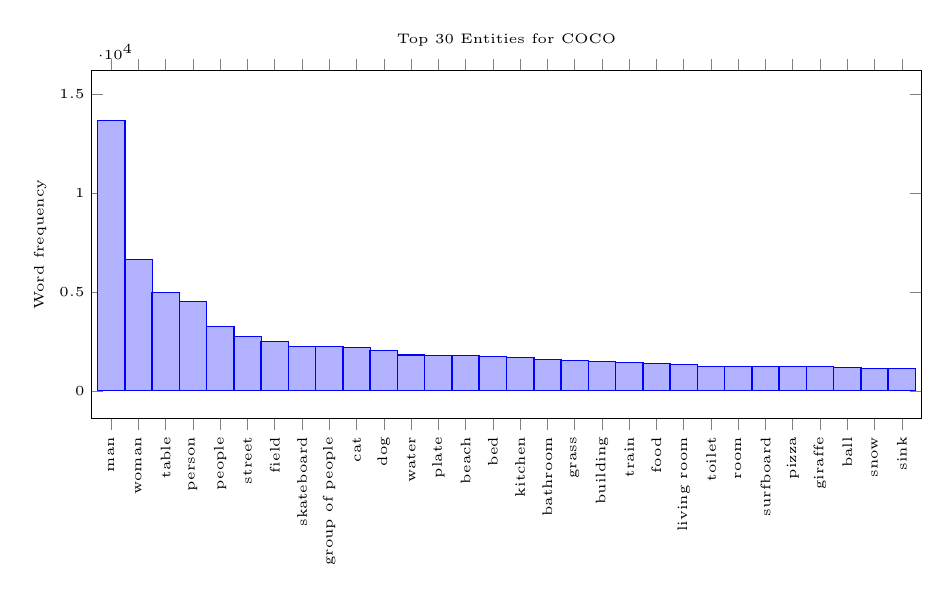
\begin{tikzpicture}
\tiny
  \begin{axis}[
    xtick=data,
    ybar,
    xlabel=Top 30 Entities for COCO,
    ylabel=Word frequency,
    width=\textwidth,
    height=6cm,
    enlarge x limits=0.025,
    enlarge y limits=0.2,
    xticklabel style={rotate=90},
    xlabel style={at={(0.5,1.05)}, anchor=south},
    symbolic x coords={man,woman,table,person,people,street,field,skateboard,group of people,cat,dog,water,plate,beach,bed,kitchen,bathroom,grass,building,train,food,living room,toilet,room,surfboard,pizza,giraffe,ball,snow,sink,}
  ]
  \addplot coordinates {
    (man, 13676)
    (woman, 6624)
    (table, 4963)
    (person, 4518)
    (people, 3228)
    (street, 2756)
    (field, 2482)
    (skateboard, 2251)
    (group of people, 2233)
    (cat, 2178)
    (dog, 2025)
    (water, 1809)
    (plate, 1795)
    (beach, 1792)
    (bed, 1750)
    (kitchen, 1679)
    (bathroom, 1563)
    (grass, 1526)
    (building, 1463)
    (train, 1444)
    (food, 1372)
    (living room, 1315)
    (toilet, 1247)
    (room, 1222)
    (surfboard, 1221)
    (pizza, 1216)
    (giraffe, 1215)
    (ball, 1176)
    (snow, 1123)
    (sink, 1118)
  };
  \end{axis}
\end{tikzpicture}
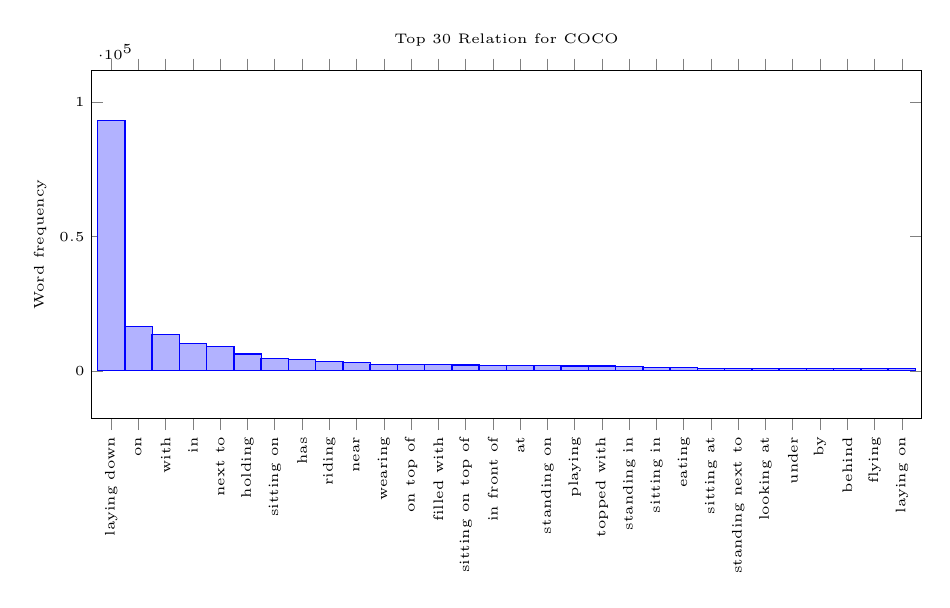
\begin{tikzpicture}
\tiny
  \begin{axis}[
    xtick=data,
    ybar,
    xlabel=Top 30 Relation for COCO,
    ylabel=Word frequency,
    width=\textwidth,
    height=6cm,
    enlarge x limits=0.025,
    enlarge y limits=0.2,
    xticklabel style={rotate=90},
    xlabel style={at={(0.5,1.05)}, anchor=south},
    symbolic x coords={laying down,on,with,in,next to,holding,sitting on,has,riding,near,wearing,on top of,filled with,sitting on top of,in front of,at,standing on,playing,topped with,standing in,sitting in,eating,sitting at,standing next to,looking at,under,by,behind,flying,laying on,}
  ]
  \addplot coordinates {
    (laying down, 93385)
    (on, 16607)
    (with, 13665)
    (in, 10224)
    (next to, 8983)
    (holding, 6307)
    (sitting on, 4772)
    (has, 4126)
    (riding, 3618)
    (near, 3254)
    (wearing, 2474)
    (on top of, 2374)
    (filled with, 2344)
    (sitting on top of, 2206)
    (in front of, 2007)
    (at, 1962)
    (standing on, 1932)
    (playing, 1832)
    (topped with, 1820)
    (standing in, 1740)
    (sitting in, 1391)
    (eating, 1390)
    (sitting at, 1052)
    (standing next to, 1031)
    (looking at, 890)
    (under, 860)
    (by, 855)
    (behind, 849)
    (flying, 831)
    (laying on, 817)
  };
  \end{axis};
\end{tikzpicture}
 \caption{Plot of the most common entities and relations that were extracted by our LLM-based parser for the COCO datasets.}
 \label{fig:coco_most_common}
\end{figure}

\begin{figure}[ht]
  \centering
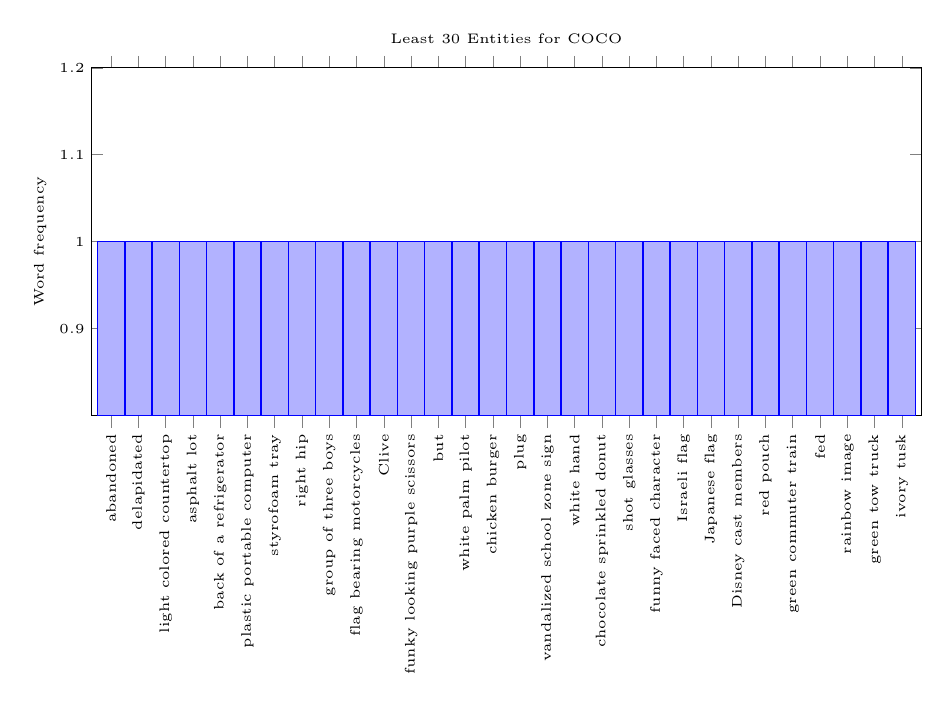
\begin{tikzpicture}
\tiny
  \begin{axis}[
    xtick=data,
    ybar,
    xlabel=Least 30 Entities for COCO,
    ylabel=Word frequency,
    width=\textwidth,
    height=6cm,
    enlarge x limits=0.025,
    enlarge y limits=0.2,
    xticklabel style={rotate=90},
    xlabel style={at={(0.5,1.05)}, anchor=south},
    symbolic x coords={abandoned,delapidated,light colored countertop,asphalt lot,back of a refrigerator,plastic portable computer,styrofoam tray,right hip,group of three boys,flag bearing motorcycles,Clive,funky looking purple scissors,but,white palm pilot,chicken burger,plug,vandalized school zone sign,white hand,chocolate sprinkled donut,shot glasses,funny faced character,Israeli flag,Japanese flag,Disney cast members,red pouch,green commuter train,fed,rainbow image,green tow truck,ivory tusk,}
  ]
  \addplot coordinates {
    (abandoned, 1)
    (delapidated, 1)
    (light colored countertop, 1)
    (asphalt lot, 1)
    (back of a refrigerator, 1)
    (plastic portable computer, 1)
    (styrofoam tray, 1)
    (right hip, 1)
    (group of three boys, 1)
    (flag bearing motorcycles, 1)
    (Clive, 1)
    (funky looking purple scissors, 1)
    (but, 1)
    (white palm pilot, 1)
    (chicken burger, 1)
    (plug, 1)
    (vandalized school zone sign, 1)
    (white hand, 1)
    (chocolate sprinkled donut, 1)
    (shot glasses, 1)
    (funny faced character, 1)
    (Israeli flag, 1)
    (Japanese flag, 1)
    (Disney cast members, 1)
    (red pouch, 1)
    (green commuter train, 1)
    (fed, 1)
    (rainbow image, 1)
    (green tow truck, 1)
    (ivory tusk, 1)
  };
  \end{axis}
\end{tikzpicture}
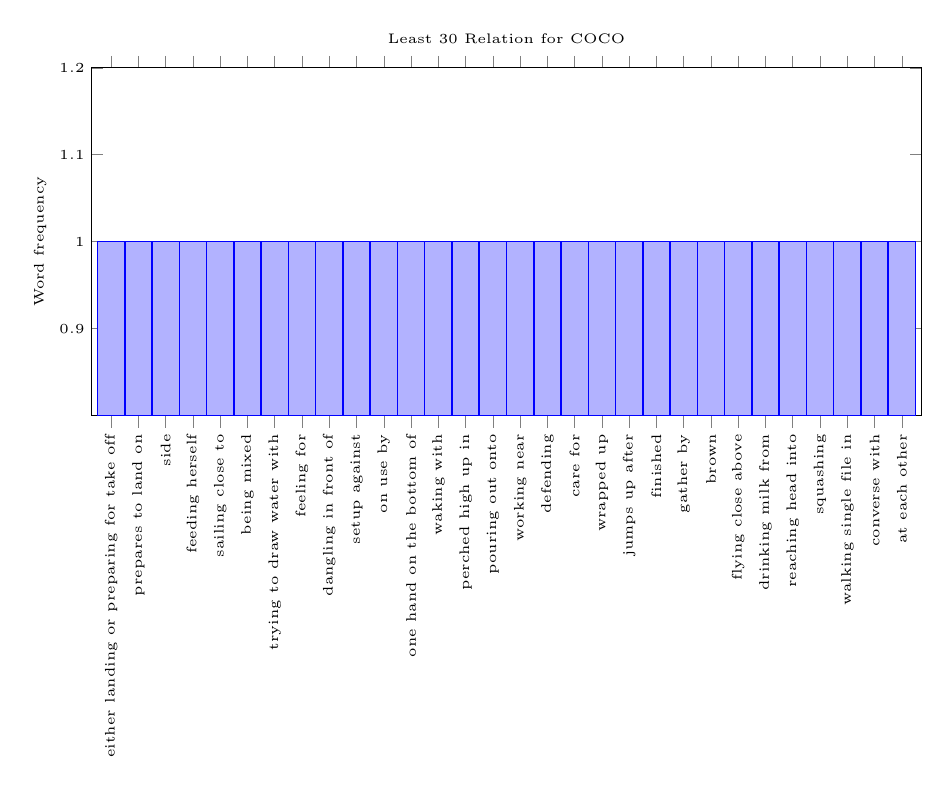
\begin{tikzpicture}
\tiny
  \begin{axis}[
    xtick=data,
    ybar,
    xlabel=Least 30 Relation for COCO,
    ylabel=Word frequency,
    width=\textwidth,
    height=6cm,
    enlarge x limits=0.025,
    enlarge y limits=0.2,
    xticklabel style={rotate=90},
    xlabel style={at={(0.5,1.05)}, anchor=south},
    symbolic x coords={either landing or preparing for take off,prepares to land on,side,feeding herself,sailing close to,being mixed,trying to draw water with,feeling for,dangling in front of,setup against,on use by,one hand on the bottom of,waking with,perched high up in,pouring out onto,working near,defending,care for,wrapped up,jumps up after,finished,gather by,brown,flying close above,drinking milk from,reaching head into,squashing,walking single file in,converse with,at each other,}
  ]
  \addplot coordinates {
    (either landing or preparing for take off, 1)
    (prepares to land on, 1)
    (side, 1)
    (feeding herself, 1)
    (sailing close to, 1)
    (being mixed, 1)
    (trying to draw water with, 1)
    (feeling for, 1)
    (dangling in front of, 1)
    (setup against, 1)
    (on use by, 1)
    (one hand on the bottom of, 1)
    (waking with, 1)
    (perched high up in, 1)
    (pouring out onto, 1)
    (working near, 1)
    (defending, 1)
    (care for, 1)
    (wrapped up, 1)
    (jumps up after, 1)
    (finished, 1)
    (gather by, 1)
    (brown, 1)
    (flying close above, 1)
    (drinking milk from, 1)
    (reaching head into, 1)
    (squashing, 1)
    (walking single file in, 1)
    (converse with, 1)
    (at each other, 1)
  };
  \end{axis}
\end{tikzpicture}
 \caption{Plot of the least common entities and relations that were extracted by our LLM-based parser for the COCO datasets.}
  \label{fig:coco_least_common}
\end{figure}

\begin{figure}[ht]
  \centering
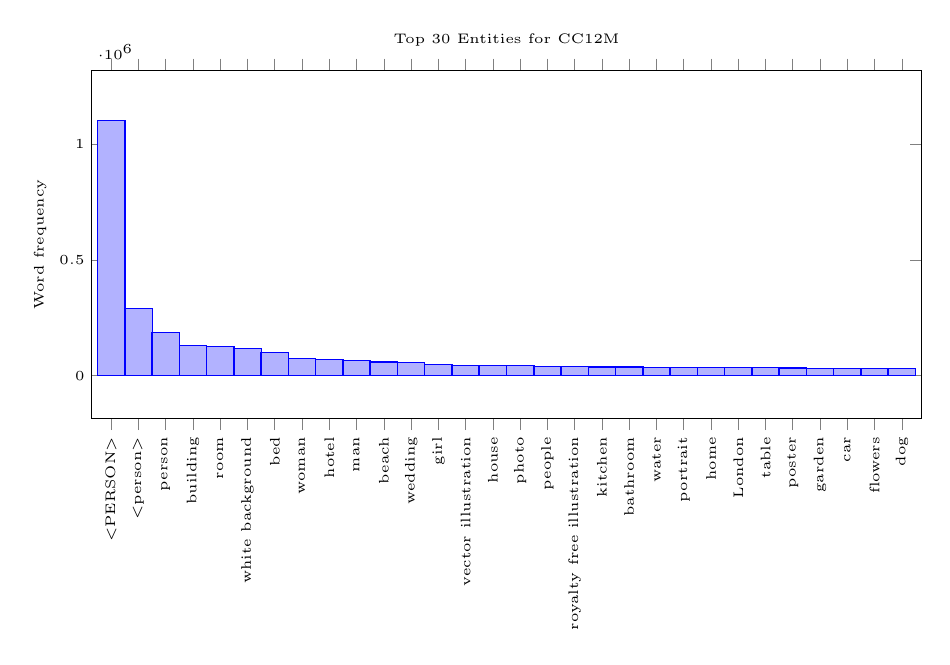
\begin{tikzpicture}
\tiny
  \begin{axis}[
    xtick=data,
    ybar,
    xlabel=Top 30 Entities for CC12M,
    ylabel=Word frequency,
    width=\textwidth,
    height=6cm,
    enlarge x limits=0.025,
    enlarge y limits=0.2,
    xticklabel style={rotate=90},
    xlabel style={at={(0.5,1.05)}, anchor=south},
    symbolic x coords={<PERSON>,<person>,person,building,room,white background,bed,woman,hotel,man,beach,wedding,girl,vector illustration,house,photo,people,royalty free illustration,kitchen,bathroom,water,portrait,home,London,table,poster,garden,car,flowers,dog,}
  ]
  \addplot coordinates {
    (<PERSON>, 1105209)
    (<person>, 290129)
    (person, 184634)
    (building, 129756)
    (room, 125712)
    (white background, 116965)
    (bed, 98864)
    (woman, 72515)
    (hotel, 69235)
    (man, 64484)
    (beach, 58818)
    (wedding, 55548)
    (girl, 47695)
    (vector illustration, 42616)
    (house, 42504)
    (photo, 42161)
    (people, 40436)
    (royalty free illustration, 38087)
    (kitchen, 37300)
    (bathroom, 37020)
    (water, 36492)
    (portrait, 36375)
    (home, 36222)
    (London, 33176)
    (table, 33110)
    (poster, 32790)
    (garden, 32373)
    (car, 32165)
    (flowers, 29948)
    (dog, 29805)
  };
  \end{axis}
\end{tikzpicture}
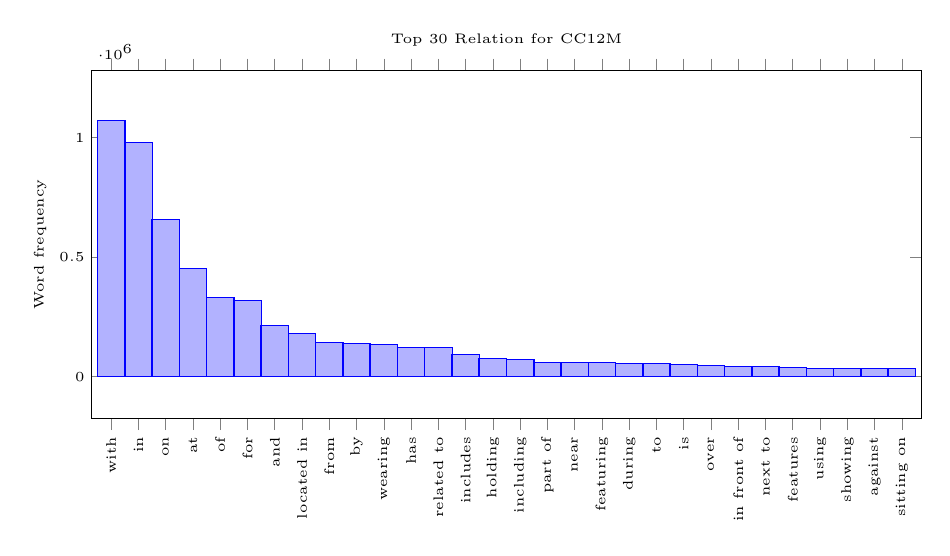
\begin{tikzpicture}
\tiny
  \begin{axis}[
    xtick=data,
    ybar,
    xlabel=Top 30 Relation for CC12M,
    ylabel=Word frequency,
    width=\textwidth,
    height=6cm,
    enlarge x limits=0.025,
    enlarge y limits=0.2,
    xticklabel style={rotate=90},
    xlabel style={at={(0.5,1.05)}, anchor=south},
    symbolic x coords={with,in,on,at,of,for,and,located in,from,by,wearing,has,related to,includes,holding,including,part of,near,featuring,during,to,is,over,in front of,next to,features,using,showing,against,sitting on,}
  ]
  \addplot coordinates {
    (with, 1073543)
    (in, 981344)
    (on, 658344)
    (at, 453675)
    (of, 329627)
    (for, 317847)
    (and, 214960)
    (located in, 179057)
    (from, 144450)
    (by, 137520)
    (wearing, 134435)
    (has, 123377)
    (related to, 122067)
    (includes, 91638)
    (holding, 74895)
    (including, 72025)
    (part of, 59609)
    (near, 59361)
    (featuring, 57766)
    (during, 55396)
    (to, 54933)
    (is, 49526)
    (over, 45001)
    (in front of, 42612)
    (next to, 40557)
    (features, 39894)
    (using, 35223)
    (showing, 34862)
    (against, 34621)
    (sitting on, 33226)
  };
  \end{axis}
\end{tikzpicture}
 \caption{Plot of the most common entities and relations that were extracted by our LLM-based parser for the CC12M dataset.}
  \label{fig:cc12m_most_common}
\end{figure}


\ifarxiv
\begin{figure}
        \centering
        \includegraphics[width=0.5\linewidth]{figures/token_freq_entities_coco.pdf}
        \includegraphics[width=0.5\linewidth]{figures/token_freq_relations_coco.pdf}
     \caption{Distribution of the number of tokens require for modeling the entities and relations on COCO (we do not need more than 8 tokens to capture 99\% of the entities in COCO). Since we need less token, we can leverage a smaller text encoder to extract the entities and relations.}
      \label{fig:coco_token_dist}
    \end{figure}

    \begin{figure}
        \centering
        \includegraphics[width=0.5\linewidth]{figures/token_freq_entities_cc12m.pdf}
        \includegraphics[width=0.5\linewidth]{figures/token_freq_relation_cc12m.pdf}
     \caption{Distribution of the number of tokens require for modeling the entities and relations on CC12M (we do not need more than 14 tokens to capture 99\% of the entities in CC12M). Since we need less token, we can leverage a smaller text encoder to extract the entities and relations.}
      \label{fig:cc12m_token_dist}
    \end{figure}
    
\else
    \begin{figure}
        \centering
        \includegraphics[width=1.0\linewidth]{figures/token_freq_entities_coco.pdf}
        \includegraphics[width=1.0\linewidth]{figures/token_freq_relations_coco.pdf}
     \caption{Distribution of the number of tokens require for modeling the entities and relations on COCO (we do not need more than 8 tokens to capture 99\% of the entities in COCO). Since we need less token, we can leverage a smaller text encoder to extract the entities and relations.}
      \label{fig:coco_token_dist}
    \end{figure}

    \begin{figure}
        \centering
        \includegraphics[width=1.0\linewidth]{figures/token_freq_entities_cc12m.pdf}
        \includegraphics[width=1.0\linewidth]{figures/token_freq_relation_cc12m.pdf}
     \caption{Distribution of the number of tokens require for modeling the entities and relations on CC12M (we do not need more than 14 tokens to capture 99\% of the entities in CC12M). Since we need less token, we can leverage a smaller text encoder to extract the entities and relations.}
      \label{fig:cc12m_token_dist}
    \end{figure}
\fi


\subsection{Datasets} 
\paragraph{Training Data}
For the compositional experiments we train both OpenCLIP and OC-CLIP on a aggregated data form COCO-Captions (COCO) \citep{coco}, Visual Genome (VG) \citep{krishna2017visual} and GQA \citep{hudson2019gqa}. All these datasets cover the same 110k images from COCO but focus on different kind of annotations. COCO provide global scene annotation, Visual Genome emphasizes specific region descriptions and general relationships and GQA annotates both objects and spatial relationships. Both Visual Genome and GQA have annotated scene graph that we do not need to parse to train OC-CLIP. For OpenCLIP, we sample 2 region annotations from VG to from a caption following this template \emph{A photo of a \{Region 1\} and a \{Region 2\}}. Similarly to get the captions from GQA, if there is a relationship we follow \citet{kamath2023whatsupvisionlanguagemodels} and give the model a caption following this template \emph{A photo of \{Subject\} \{Rel\} \{Object\}}. If only objects are mentionned we sample up to 3 objects and give the model a caption following this template \emph{A photo of \{Obj1\},\{Obj2\},\{ Obj3\} }.
\subsection{Training Details and Hyperparameters}

In table \ref{tab:hyperparam} we detail the hyperparameters of the OC-CLIP architecture for results in real-world compositional understanding (section 4.2).
\paragraph{Optimization Details} In order to train OC-CLIP we followed prior work and use Adam Optimizer with $\beta_1$ and $\beta_2$ set to 0.9 and 0.95 and a weight decay of 0.2. We used different learning rate for the pretrained backbones and for our modules that we train from scratch : learning rate of $2e^{-4}$ for the binding and the scoring modules, learning rate of $2e^{-5}$ for the text Transformer backbone, and a smaller rate of $1e^{-6}$ for the ViT backbone. We also used a warmup schedule for both of the text (1k steps) and the vision (5k steps) backbones followed by a cosine decay. We train the model for a total of 100 epochs. 
\begin{table}[ht]
\centering
\begin{tabular}{@{}lccc@{}}
\toprule
Hyperparameter/Parameter Init & Architecture & Value\\ 
\midrule
\textbf{Binding Module} &  &  & \\
-- Image Patches Processing & Linear & 768 $\times$ 256 & \\
-- Self-Attention  \#Layers/\#Heads &  & 2/4 & \\
-- Self-Attention MLP ratio/act &  & 2/nn.GELU & \\
-- Keys $K$, Values $V$ & Linear & 256, 256 & \\
-- Normalization Keys/Values & LayerNorm & 256 & \\
\midrule
\textbf{Grouping Module} &  &  & \\
-- Cross-Attention \#Heads &  & 1 & \\
-- Queries & Linear & 256 \\
-- Normalization Queries & LayerNorm & 256 \\
-- Num Default Tokens $Q_{\text{default}}$ & nn.Param($N_d$,256) & 1\\
\midrule
\textbf{Scoring Functions} &  &  & \\

-- Object Scoring Function & cosine sim  &  & \\
-- Relation Scoring subject $ f_s$ &  MLP(128 + 256, 128) & 2 layers & \\
-- Relation Scoring object $ f_o$ &  MLP(128 + 256, 128) & 2 layers & \\
-- Coef ent init (learned parameter) & &1.5 \\
-- Coef rel init (learned parameter) & & 0.5\\

 \bottomrule
\end{tabular}%
% }
\caption{Table of hyperparameters for OC-CLIP architecture}
\label{tab:hyperparam}
\end{table}

\ifarxiv
\else
\vspace{-20pt}
\fi
%\subsection{Attention maps}
%See Figure~\ref{fig:attn}
\iffalse
\begin{figure}[h]
\centering
\begin{minipage}{\textwidth}
  \centering
  \includegraphics[width=\linewidth]{figures/attn_pug_1.pdf}
  \caption{A photo of a white lion and an asphalt penguin in a circus. }
\end{minipage}
\begin{minipage}{\textwidth}
  \centering
  \includegraphics[width=\linewidth]{figures/attn_pug_2.pdf}
  \caption{A photo of a white bear and a rhinoceros in a arena.}
\end{minipage}
\begin{minipage}{\textwidth}
  \centering
  \includegraphics[width=\linewidth]{figures/attn_pug_3.pdf}
  \caption{A photo of an asphalt orca and a red lion in a city.}
\end{minipage}
\begin{minipage}{\textwidth}
  \centering
  \includegraphics[width=\linewidth]{figures/attn_pug_4.pdf}
  \caption{A photo of a white bear and a red gianttortoise in a circus.}
\end{minipage}
\begin{minipage}{\textwidth}
  \centering
  \includegraphics[width=\linewidth]{figures/attn_pug_5.pdf}
  \caption{A photo of a red crow and an asphalt zebra in a ocean floor.}
\end{minipage}
\caption{OC-CLIP Binding Attention Maps on PUG. We plot the attention maps of each query object in the caption (specified at the top of each attention map) and notice that natural objects emerge.}
\label{fig:attn}
\end{figure}
\fi

\subsection{Binding Module Code}
See Figure \ref{fig:code}

\begin{figure}
    \centering
    \includegraphics[width=\linewidth]{figures/code.png}
    \caption{Code for the Binding Module}
    \label{fig:code}
\end{figure}

%\begin{listing}[h]
    %\begin{minted}{python}
    % class AssignAttention(nn.Module) : 
    %     def __init__(
    %         self, dim, qkv_bias=False, qk_scale=None):
    %         super().__init__()
    %         self.scale = qk_scale or dim**-0.5
    %         self.q_proj = nn.Sequential(nn.Linear(dim, dim, bias=qkv_bias))
    %         self.k_proj = nn.Sequential(nn.Linear(dim, dim, bias=qkv_bias))
    %         self.v_proj = nn.Sequential(nn.Linear(dim, dim, bias=qkv_bias))
    
    %     def forward(self, query, key=None, value=None):
    %         #before cross attention projections
    %         q = self.q_proj(query)
    %         k = self.k_proj(key)
    %         v = self.v_proj(value)
    %         #scaled dot product
    %         attn = (q @ k.transpose(-2, -1)) * self.scale
    %         #softmax across query dim
    %         attn_dim = -2
    %         attn = F.softmax(attn, dim=attn_dim) + 1e-8 
    %         #attn normoalization
    %         attn = attn / (attn.sum(dim=-1, keepdim=True)) 
    %         output = torch.einsum("bqk,bkd->bqd", attn, v) 
    %         return output
    % class BindingModule(nn.Module) :
    %     def __init__(self,in_vis_dim, dim, num_patches, num_default_tokens) : 
    %         super().__init__()
    %         self.im_proj = nn.Sequential(nn.Linear(in_vis_dim, dim), 
    %         nn.GELU(), nn.Linear(dim, dim))
    %         self.pos_embeddings = nn.Parameter(torch.randn(num_patches, dim))
    %         self.img_processor = nn.Sequential( ResidualAttnBlock(dim, 4),
    %         ResidualAttnBlock(dim, 4))
    %         self.default_tokens = nn.Parameter(
    %         torch.randn(1, num_default_tokens, dim))
    %         self.to_kq_groups = nn.Sequential(nn.Linear(dim, 2 * dim))
    %         self.dim = dim
    %         self.num_default_tokens = num_default_tokens
    %         self.k_norm = nn.LayerNorm(dim)
    %         self.v_norm = nn.LayerNorm(dim)
    %         self.assign_slots = AssignAttention(dim)
        
    %     def encode_patches(self, patches) : 
    %         patches = self.im_proj(patches)
    %         patches = patches + self.pos_embeddings
    %         patches = self.img_processor(patches)
    %         K_img, V_img = torch.split(
    %         self.to_kq_groups(patches),self.dim,dim=-1)
    %         K_img, V_img = self.k_norm(K_img), self.v_norm(V_img)
    %         return K_img, V_img
        
    %     def group(self, query_tokens, K_img, V_img) : 
    %         #adding default tokens
    %         query_tokens= torch.cat([query_tokens,default_tokens ], 1)
    %         out = self.assign_slots(query_tokens, K_img, V_img)
    %         #remove default tokens
    %         out = out[:, :-self.num_default_tokens] 
    %         return out
        
    % \end{minted}
%\end{listing}

\begin{figure}[ht]
  \centering
    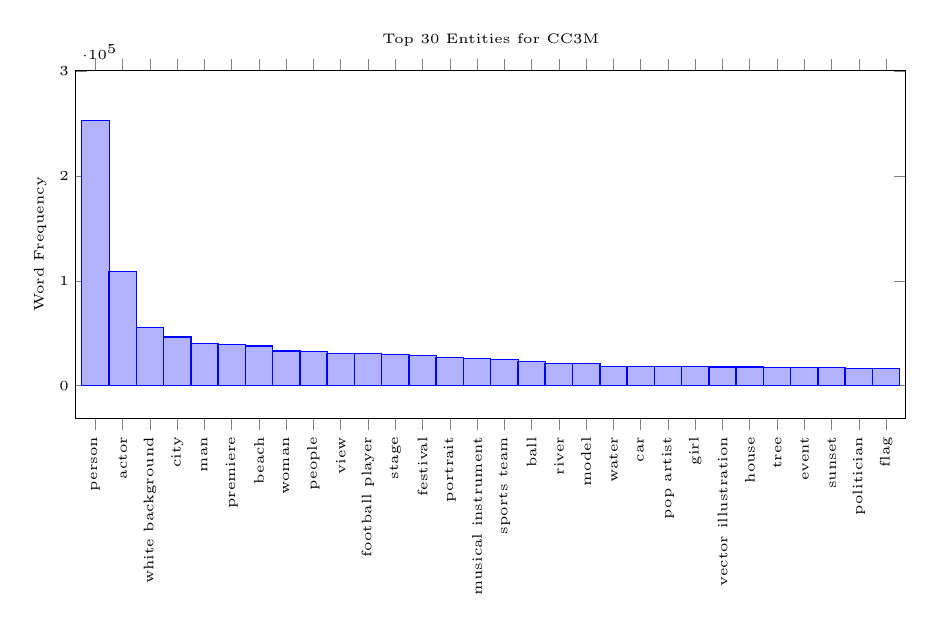
\begin{tikzpicture}
    \tiny
      \begin{axis}[
        xtick=data,
        ybar,
        xlabel=Top 30 Entities for CC3M,
        ylabel=Word Frequency,
        width=\textwidth,
        height=6cm,
        enlarge x limits=0.025,
        enlarge y limits=0.2,
        xticklabel style={rotate=90},
        xlabel style={at={(0.5,1.05)}, anchor=south},
        symbolic x coords={person,actor,white background,city,man,premiere,beach,woman,people,view,football player,stage,festival,portrait,musical instrument,sports team,ball,river,model,water,car,pop artist,girl,vector illustration,house,tree,event,sunset,politician,flag,}
      ]
      \addplot coordinates {
        (person, 253338)
        (actor, 109367)
        (white background, 55313)
        (city, 46557)
        (man, 40357)
        (premiere, 39363)
        (beach, 37933)
        (woman, 33204)
        (people, 32698)
        (view, 31104)
        (football player, 30497)
        (stage, 30222)
        (festival, 29221)
        (portrait, 26613)
        (musical instrument, 25862)
        (sports team, 25470)
        (ball, 23177)
        (river, 21091)
        (model, 20986)
        (water, 18405)
        (car, 18364)
        (pop artist, 18161)
        (girl, 18079)
        (vector illustration, 17925)
        (house, 17882)
        (tree, 17764)
        (event, 17721)
        (sunset, 17632)
        (politician, 16641)
        (flag, 16300)
      };
    \end{axis}
    \end{tikzpicture}
    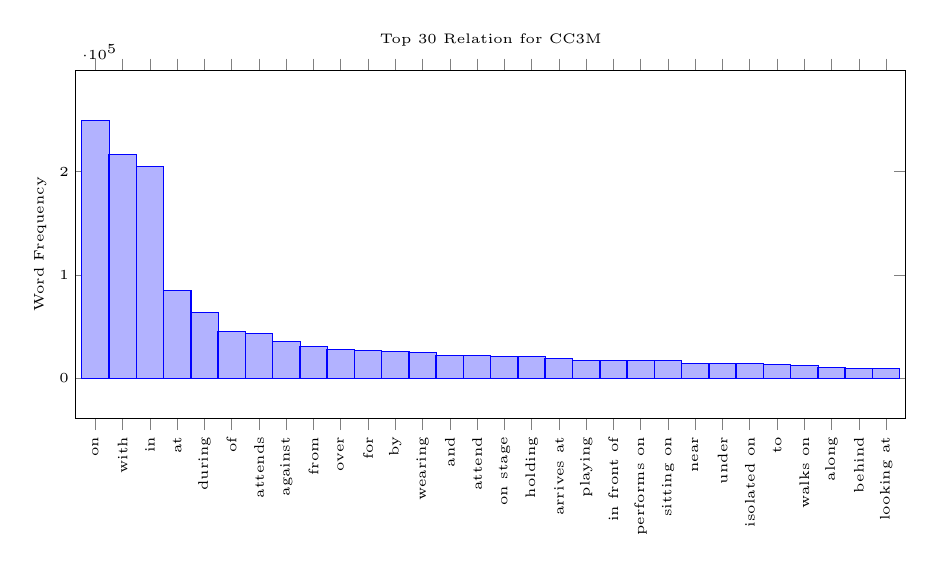
\begin{tikzpicture}
    \tiny
      \begin{axis}[
        xtick=data,
        ybar,
        xlabel=Top 30 Relation for CC3M,
        ylabel=Word Frequency,
        width=\textwidth,
        height=6cm,
        enlarge x limits=0.025,
        enlarge y limits=0.2,
        xticklabel style={rotate=90},
        xlabel style={at={(0.5,1.05)}, anchor=south},
        symbolic x coords={on,with,in,at,during,of,attends,against,from,over,for,by,wearing,and,attend,on stage,holding,arrives at,playing,in front of,performs on,sitting on,near,under,isolated on,to,walks on,along,behind,looking at,}
      ]
      \addplot coordinates {
        (on, 249858)
        (with, 216254)
        (in, 205332)
        (at, 85210)
        (during, 64058)
        (of, 45280)
        (attends, 43674)
        (against, 35350)
        (from, 30801)
        (over, 27717)
        (for, 26672)
        (by, 25561)
        (wearing, 25397)
        (and, 22231)
        (attend, 22125)
        (on stage, 21332)
        (holding, 21096)
        (arrives at, 19263)
        (playing, 17608)
        (in front of, 17030)
        (performs on, 16946)
        (sitting on, 16848)
        (near, 14713)
        (under, 14603)
        (isolated on, 14316)
        (to, 13172)
        (walks on, 12068)
        (along, 10332)
        (behind, 9357)
        (looking at, 9337)
      };
    \end{axis}
    \end{tikzpicture}
 \caption{Top entities and relation for CC3M}
\end{figure}

\begin{figure}[ht]
  \centering
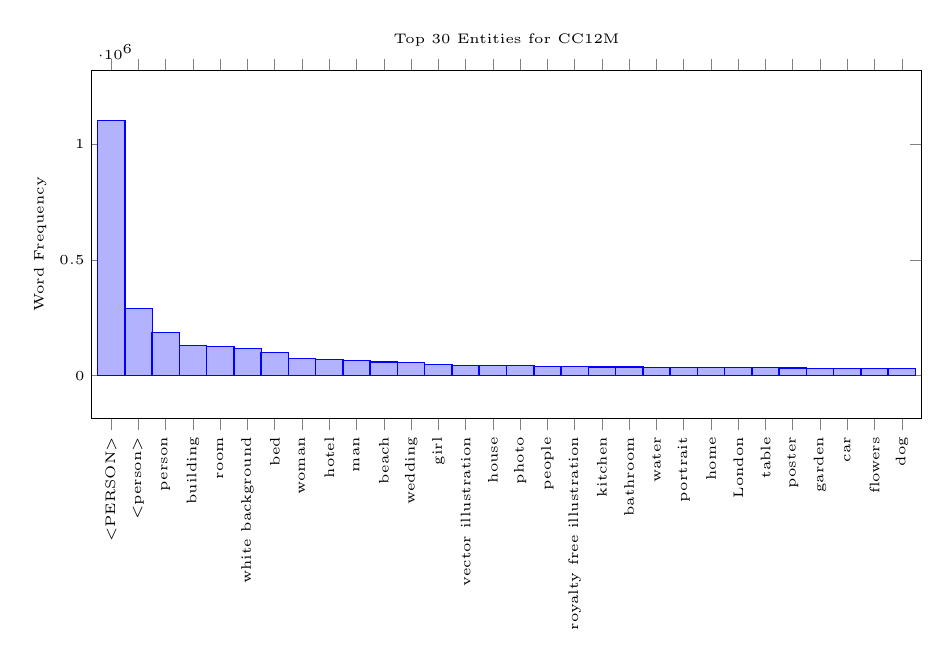
\begin{tikzpicture}
\tiny
  \begin{axis}[
    xtick=data,
    ybar,
    xlabel=Top 30 Entities for CC12M,
    ylabel=Word Frequency,
    width=\textwidth,
    height=6cm,
    enlarge x limits=0.025,
    enlarge y limits=0.2,
    xticklabel style={rotate=90},
    xlabel style={at={(0.5,1.05)}, anchor=south},
    symbolic x coords={<PERSON>,<person>,person,building,room,white background,bed,woman,hotel,man,beach,wedding,girl,vector illustration,house,photo,people,royalty free illustration,kitchen,bathroom,water,portrait,home,London,table,poster,garden,car,flowers,dog,}
  ]
  \addplot coordinates {
    (<PERSON>, 1105209)
    (<person>, 290129)
    (person, 184634)
    (building, 129756)
    (room, 125712)
    (white background, 116965)
    (bed, 98864)
    (woman, 72515)
    (hotel, 69235)
    (man, 64484)
    (beach, 58818)
    (wedding, 55548)
    (girl, 47695)
    (vector illustration, 42616)
    (house, 42504)
    (photo, 42161)
    (people, 40436)
    (royalty free illustration, 38087)
    (kitchen, 37300)
    (bathroom, 37020)
    (water, 36492)
    (portrait, 36375)
    (home, 36222)
    (London, 33176)
    (table, 33110)
    (poster, 32790)
    (garden, 32373)
    (car, 32165)
    (flowers, 29948)
    (dog, 29805)
  };
  \end{axis}
\end{tikzpicture}
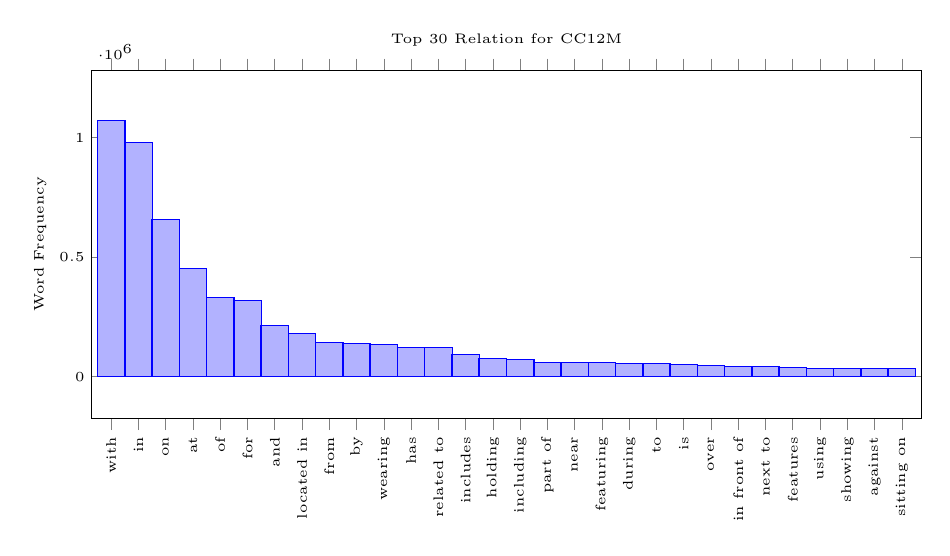
\begin{tikzpicture}
\tiny
  \begin{axis}[
    xtick=data,
    ybar,
    xlabel=Top 30 Relation for CC12M,
    ylabel=Word Frequency,
    width=\textwidth,
    height=6cm,
    enlarge x limits=0.025,
    enlarge y limits=0.2,
    xticklabel style={rotate=90},
    xlabel style={at={(0.5,1.05)}, anchor=south},
    symbolic x coords={with,in,on,at,of,for,and,located in,from,by,wearing,has,related to,includes,holding,including,part of,near,featuring,during,to,is,over,in front of,next to,features,using,showing,against,sitting on,}
  ]
  \addplot coordinates {
    (with, 1073543)
    (in, 981344)
    (on, 658344)
    (at, 453675)
    (of, 329627)
    (for, 317847)
    (and, 214960)
    (located in, 179057)
    (from, 144450)
    (by, 137520)
    (wearing, 134435)
    (has, 123377)
    (related to, 122067)
    (includes, 91638)
    (holding, 74895)
    (including, 72025)
    (part of, 59609)
    (near, 59361)
    (featuring, 57766)
    (during, 55396)
    (to, 54933)
    (is, 49526)
    (over, 45001)
    (in front of, 42612)
    (next to, 40557)
    (features, 39894)
    (using, 35223)
    (showing, 34862)
    (against, 34621)
    (sitting on, 33226)
  };
  \end{axis}
\end{tikzpicture}
 \caption{Top entities and relation for CC12M}
\end{figure}

\begin{figure}[ht]
  \centering
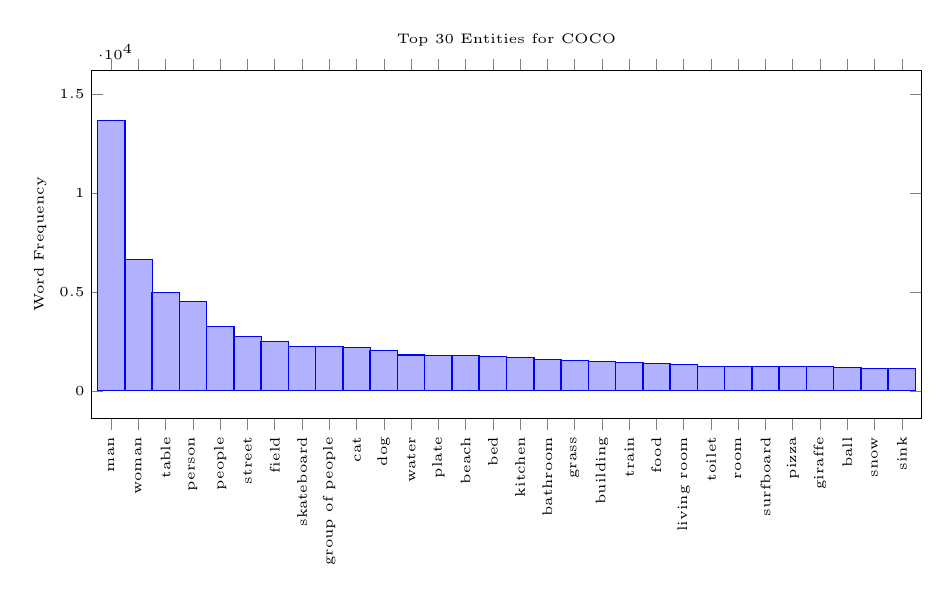
\begin{tikzpicture}
\tiny
  \begin{axis}[
    xtick=data,
    ybar,
    xlabel=Top 30 Entities for COCO,
    ylabel=Word Frequency,
    width=\textwidth,
    height=6cm,
    enlarge x limits=0.025,
    enlarge y limits=0.2,
    xticklabel style={rotate=90},
    xlabel style={at={(0.5,1.05)}, anchor=south},
    symbolic x coords={man,woman,table,person,people,street,field,skateboard,group of people,cat,dog,water,plate,beach,bed,kitchen,bathroom,grass,building,train,food,living room,toilet,room,surfboard,pizza,giraffe,ball,snow,sink,}
  ]
  \addplot coordinates {
    (man, 13676)
    (woman, 6624)
    (table, 4963)
    (person, 4518)
    (people, 3228)
    (street, 2756)
    (field, 2482)
    (skateboard, 2251)
    (group of people, 2233)
    (cat, 2178)
    (dog, 2025)
    (water, 1809)
    (plate, 1795)
    (beach, 1792)
    (bed, 1750)
    (kitchen, 1679)
    (bathroom, 1563)
    (grass, 1526)
    (building, 1463)
    (train, 1444)
    (food, 1372)
    (living room, 1315)
    (toilet, 1247)
    (room, 1222)
    (surfboard, 1221)
    (pizza, 1216)
    (giraffe, 1215)
    (ball, 1176)
    (snow, 1123)
    (sink, 1118)
  };
  \end{axis}
\end{tikzpicture}
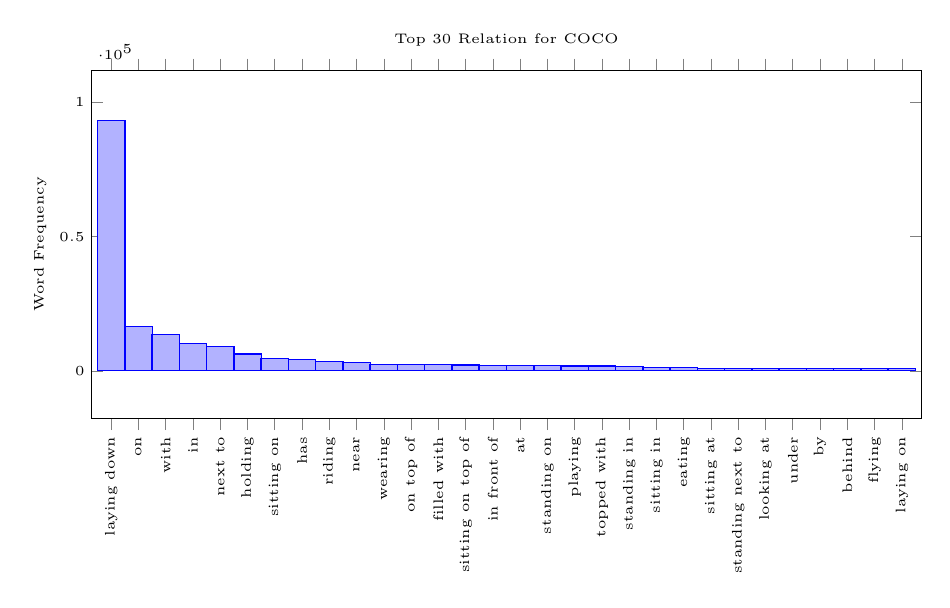
\begin{tikzpicture}
\tiny
  \begin{axis}[
    xtick=data,
    ybar,
    xlabel=Top 30 Relation for COCO,
    ylabel=Word Frequency,
    width=\textwidth,
    height=6cm,
    enlarge x limits=0.025,
    enlarge y limits=0.2,
    xticklabel style={rotate=90},
    xlabel style={at={(0.5,1.05)}, anchor=south},
    symbolic x coords={laying down,on,with,in,next to,holding,sitting on,has,riding,near,wearing,on top of,filled with,sitting on top of,in front of,at,standing on,playing,topped with,standing in,sitting in,eating,sitting at,standing next to,looking at,under,by,behind,flying,laying on,}
  ]
  \addplot coordinates {
    (laying down, 93385)
    (on, 16607)
    (with, 13665)
    (in, 10224)
    (next to, 8983)
    (holding, 6307)
    (sitting on, 4772)
    (has, 4126)
    (riding, 3618)
    (near, 3254)
    (wearing, 2474)
    (on top of, 2374)
    (filled with, 2344)
    (sitting on top of, 2206)
    (in front of, 2007)
    (at, 1962)
    (standing on, 1932)
    (playing, 1832)
    (topped with, 1820)
    (standing in, 1740)
    (sitting in, 1391)
    (eating, 1390)
    (sitting at, 1052)
    (standing next to, 1031)
    (looking at, 890)
    (under, 860)
    (by, 855)
    (behind, 849)
    (flying, 831)
    (laying on, 817)
  };
 \end{axis}
\end{tikzpicture}
 \caption{Top entities and relation for COCO}
\end{figure}
